\section{Experimental Evaluation}

\subsection{Experimental Setup}

Each benchmark graph was generated using a fixed random
seed of 5405. A directed chain from the source to the sink
was included to guarantee a source-to-sink path. In addition,
approximately $4n$ random endpoint pairs were generated,
with endpoints ordered to produce forward edges and
self-loops discarded. Parallel edges were permitted.
Capacities were independently assigned from the integer
range 1 to 100. The graph was generated once for each
benchmark size and reused across the seven timed
executions. Graph construction was excluded from the
measured interval.

The experiments were conducted using C++ implementations of the
algorithms. The maximum-flow implementation uses Dinic's algorithm,
while the Bin Packing implementation uses First Fit Decreasing
(FFD) with a segment tree to accelerate bin selection.

The experiments were conducted on an Apple MacBook Pro
equipped with an Apple M1 Pro processor and running macOS
(Darwin 25.6.0) on the ARM64 architecture. The code was
compiled using Apple Clang 21.0.0
(compiler build clang-2100.1.1.101) with the CMake
Release configuration. The project build completed
successfully for the main executable, test executable,
and benchmark target.

\subsection{Maximum-Flow Experimental Results}

The maximum-flow implementation was evaluated on sparse directed
networks of increasing size. Each benchmark instance contained a
guaranteed source-to-sink path and additional edges generated
deterministically using a fixed random seed. The edge capacities
were drawn from the range 1 to 100. The graph generation procedure
was performed outside the timed execution.

Table~\ref{tab:flow_results} presents the median execution times.

\begin{table}[htbp]
\centering
\caption{Maximum-flow benchmark results}
\label{tab:flow_results}
\begin{tabular}{r r r}
\toprule
Vertices & Edges & Median (ms) \\
\midrule
1,000  & 4,996  & 1.14533 \\
2,000  & 9,997  & 1.91275 \\
4,000  & 19,994 & 4.25363 \\
8,000  & 39,993 & 19.46120 \\
12,000 & 59,999 & 39.40120 \\
\bottomrule
\end{tabular}
\end{table}

Figure~\ref{fig:flow_runtime} visualizes the measured runtime as
the network size increases.

\begin{figure}[htbp]
\centering
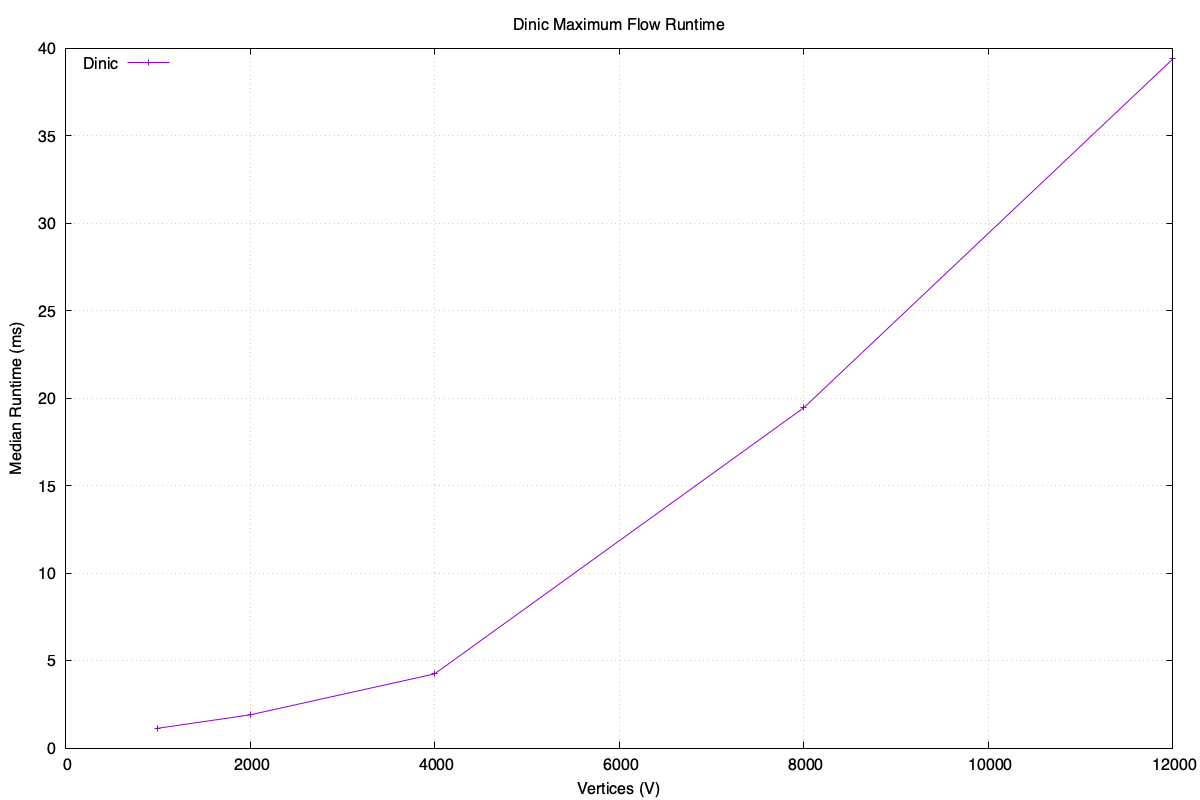
\includegraphics[width=\linewidth]{flow_runtime.png}
\caption{Measured runtime of Dinic's maximum-flow implementation
on sparse benchmark networks.}
\label{fig:flow_runtime}
\end{figure}

The measured runtime increases as the size of the network grows.
Although the benchmark networks are sparse and the number of edges
grows approximately linearly with the number of vertices, the
observed execution time does not increase linearly across the
tested sizes.

The larger instances require progressively more computation.
This behavior is consistent with the fact that Dinic's algorithm
can require substantial computational effort on general directed
networks. Its general worst-case time complexity is
$O(V^2E)$, although actual execution time depends on network
structure, capacity distribution, and the sequence of blocking
flows computed by the algorithm.

The values in the benchmark are empirical measurements and do not
establish the theoretical complexity of the algorithm.

\subsection{Bin Packing Experimental Results}

For each benchmark size, a workload instance was generated
using the random seed 5406. Item sizes were uniformly
generated as integers in the interval $[1,1000]$, and
the bin capacity was set to 1000. The generated instance
was reused across seven executions. Each timed execution
included the First Fit Decreasing routine, including sorting
and placement. Input generation was excluded from the
timed interval, and the median runtime was recorded.

The implementation sorts the items in nonincreasing order and
uses a segment tree to identify the earliest bin with sufficient
remaining capacity. Table~\ref{tab:binpack_results} summarizes
the measured median execution times.

\begin{table}[htbp]
\centering
\caption{First Fit Decreasing benchmark results}
\label{tab:binpack_results}
\begin{tabular}{r r}
\toprule
Items & Median (ms) \\
\midrule
1,000  & 0.070125 \\
2,000  & 0.167167 \\
4,000  & 0.405833 \\
8,000  & 0.859250 \\
16,000 & 1.849710 \\
32,000 & 3.924580 \\
\bottomrule
\end{tabular}
\end{table}

Figure~\ref{fig:binpack_runtime} presents the runtime as a function
of the number of items.

\begin{figure}[htbp]
\centering
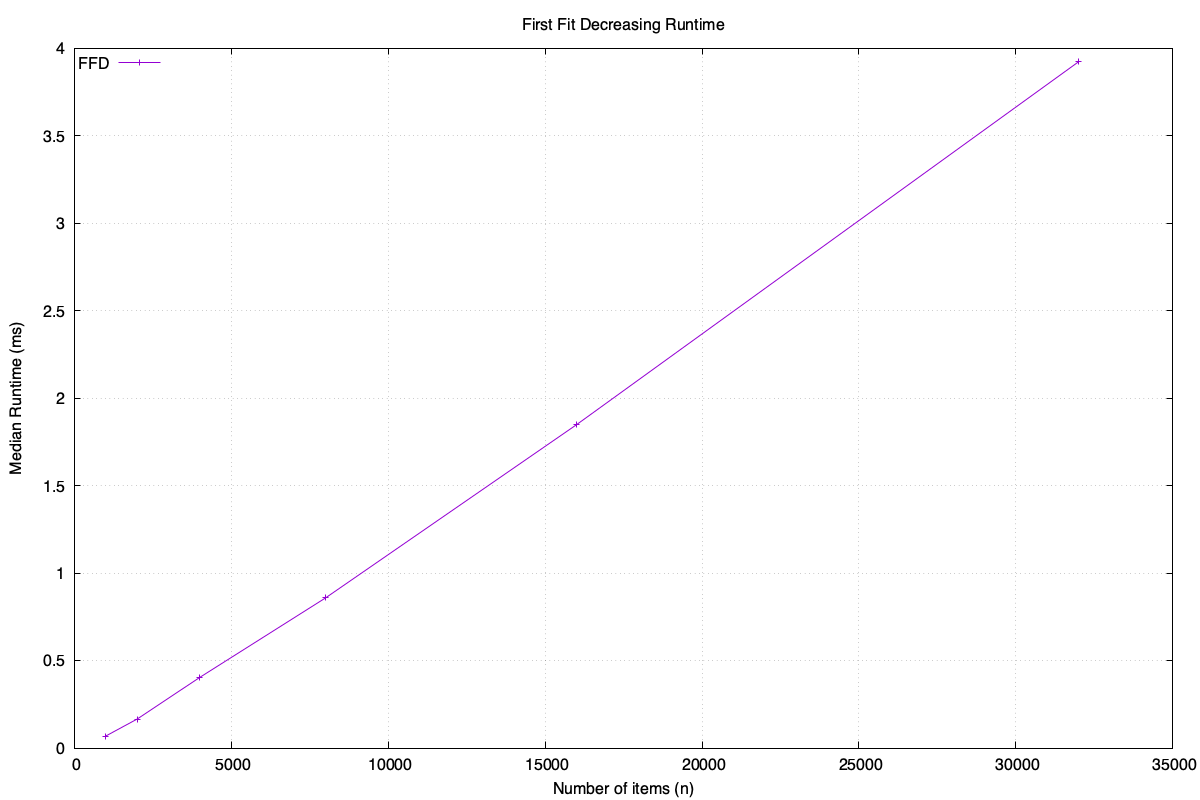
\includegraphics[width=\linewidth]{binpack_runtime.png}
\caption{Measured runtime of the First Fit Decreasing
implementation using a segment tree.}
\label{fig:binpack_runtime}
\end{figure}

The runtime increases as the number of items grows. Despite
doubling the input size at successive benchmark levels, the
observed execution times remain relatively low for the tested
instances. The implementation performs sorting in
$O(n\log n)$ time and subsequently processes each item using
segment-tree queries and updates, each requiring
$O(\log n)$ time.

Consequently, the total algorithmic runtime is
$O(n\log n)$, with $O(n)$ auxiliary storage. The measured results
are consistent with an efficient implementation of this
complexity, although empirical measurements alone cannot prove
the asymptotic bound.

\subsection{Runtime Scaling Comparison}

To further examine the scaling behavior of the Bin Packing
implementation, the measured runtime was compared with the
$n\log_2 n$ growth function.

Figure~\ref{fig:binpack_nlogn} presents this comparison.

\begin{figure}[htbp]
\centering
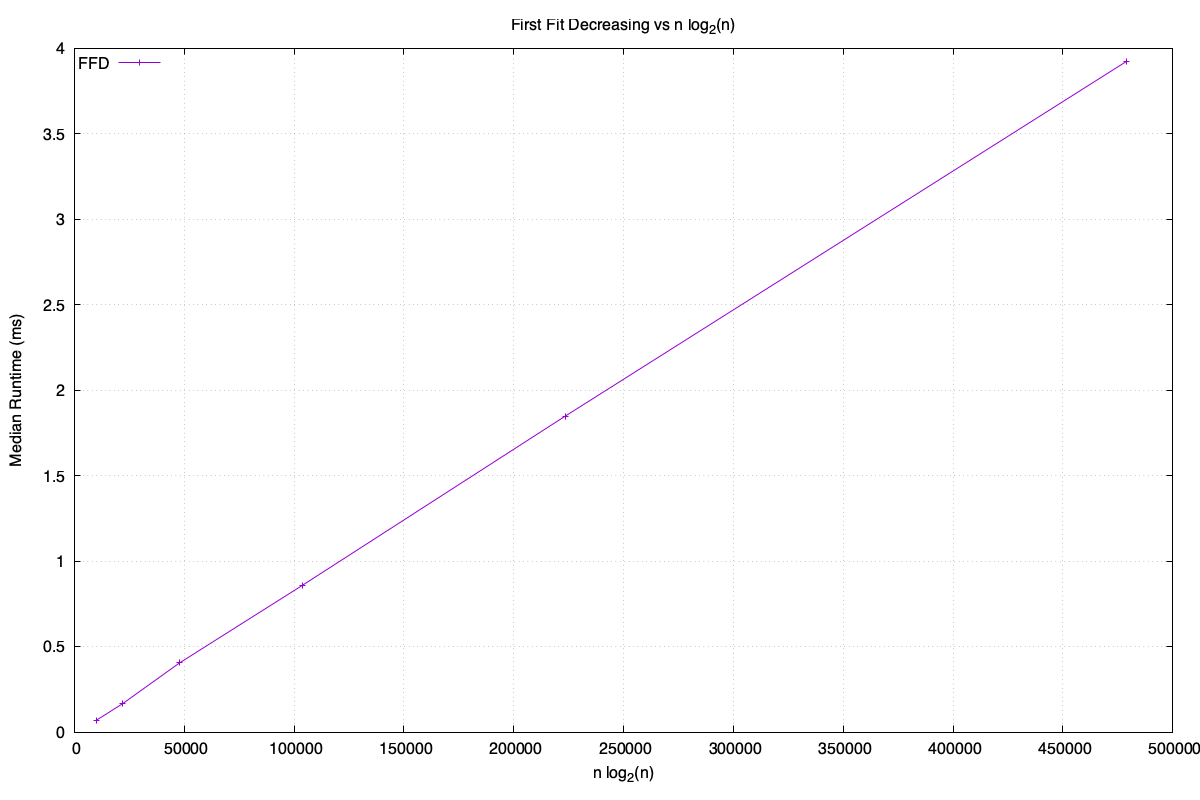
\includegraphics[width=\linewidth]{binpack_runtime_nlogn.png}
\caption{Bin Packing runtime and the $n\log_2 n$ scaling
comparison.}
\label{fig:binpack_nlogn}
\end{figure}

The comparison provides a visual reference for the expected
growth of the implementation's runtime. The $n\log_2 n$
function is used as a scaling reference rather than a direct
prediction of execution time, since it is not calibrated to the
hardware, compiler, or implementation constants.

The observed results illustrate the practical scalability of
the segment-tree-based FFD implementation over the tested input
sizes.